\usetikzlibrary{calc}
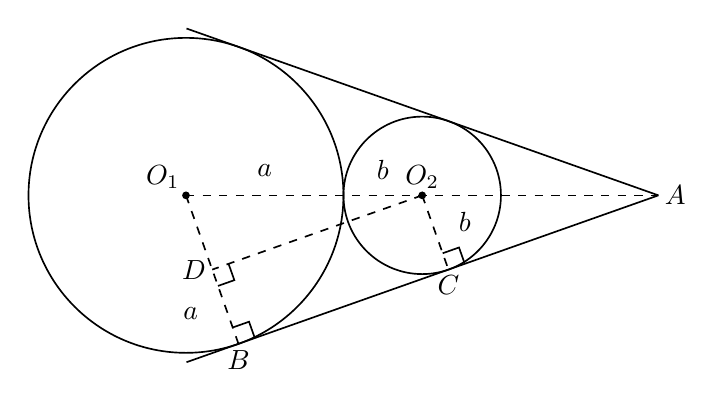
\begin{tikzpicture}[x=1cm,y=1cm,line width=.6pt,font=\normalsize]
\coordinate (O1) at (0.0000,0.0000);
\coordinate (O2) at (3.0000,0.0000);
\coordinate (T) at (2.0000,0.0000);
\coordinate (A) at (6.0000,0.0000);
\coordinate (B) at (0.6667,-1.8856);
\coordinate (C) at (3.3333,-0.9428);
\coordinate (B2) at (0.6667,1.8856);
\coordinate (C2) at (3.3333,0.9428);
\coordinate (D) at (0.3333,-0.9428);
\draw (O1) circle[radius=2.0000];
\draw (O2) circle[radius=1.0000];
\draw[dashed] (O1)--(A);
\draw (A)--(0.0067,-2.1190);
\draw (A)--(0.0067,2.1190);
\draw[dashed] (O1)--(B);
\draw[dashed] (O2)--(C);
\draw[dashed] (O2)--(D);
\draw (0.8741,-1.8123)--(0.8008,-1.6049)--(0.5933,-1.6782);
\draw (3.5408,-0.8695)--(3.4674,-0.6621)--(3.2600,-0.7354);
\draw (0.4067,-1.1502)--(0.6141,-1.0769)--(0.5408,-0.8695);
\node[above left=2pt,inner sep=0pt] at (O1) {$O_1$};
\node[above=2pt,inner sep=0pt] at (O2) {$O_2$};
\node[right=2pt,inner sep=0pt] at (A) {$A$};
\node[below=2pt,inner sep=0pt] at (B) {$B$};
\node[below=2pt,inner sep=0pt] at (C) {$C$};
\node[left=2pt,inner sep=0pt] at (D) {$D$};
\node at (0.0600,-1.5000) {$a$};
\node at (3.5400,-0.3400) {$b$};
\node at (1.0000,0.3200) {$a$};
\node at (2.5000,0.3200) {$b$};

% Explicit named circle-center points, painted after all region fills.
\fill (O1) circle[radius=1.4pt];
\fill (O2) circle[radius=1.4pt];
\end{tikzpicture}
